\chapter{Contribution}

Definition of Binder et al. \cite{binder_definitions_2022} is promising, however the branch prediction and the related issues are not taken in account by the framework. Thus we aim to extend the use case of proposed definition.

In our work we try to adjust Binder's definition to the setting of pipeline with branch predictor. We introduce an input format capable of expressing speculative execution. 

\TODO{complete intro when chapter is done}

\section{Methodology}
To systematically investigate timing anomalies induced by branch predictors, it is essential to efficiently generate and analyze relevant examples. Manual construction of such examples is both time-consuming and error-prone, motivating the need for a tool that can automatically or semi-automatically produce and validate them. With such a tool, we can iteratively generate candidate scenarios, analyze their behavior, and assess the applicability of Binder et al.'s definition to these new cases. This process enables us to refine and adapt the definition as necessary, guided by empirical evidence from the generated examples.

Our initial efforts focused on studying and extending the TLA$^+$ \cite{lamport_specifying_2003} framework developed by Binder et al.  to support branch behavior. However, we encountered significant performance limitations and found the input format insufficiently flexible for rapid prototyping and adjustment of examples.

Consequently, we reimplemented the framework in C++, drawing on insights from the TLA$^+$ model. We also use TLA$^+$ as a reference to check the correctness. The new implementation offers substantial performance improvements and introduces randomized search capabilities, enabling efficient exploration of the space of possible instruction traces and facilitating the discovery of timing anomalies related to branch prediction.

\section{Framework}

\subsection{Existing Framework Overview}

\subsubsection{Exploration by Model Checking}

The implementation provided by Binder is written in TLA$^+$ \cite{lamport_specifying_2003}. The pipeline state is specified in set-theory notation. The model checker step corresponds to a one clock cycle and derives a new HW state from the previous one. This allows to simulate the non-deterministic timing behavior: each time when a variation can happen, multiple next state are generated. TLA$^+$ covers all reachable states ensuring that all possible behaviors are covered.

The pair of trace constitutes a whole model state. TA is expressed as an invariant for the pair of traces, so its is verified in each model checking step. 

As well as a construction of traces, the framework provides visualization methods for the traces and ETDG.

% \TODO{each pair of executions is considered? or all executions are compared against the one reference?}

\subsubsection{Input Trace Format}

The input of the framework is a pair of:
\begin{enumerate}
	\item Pipeline parameters: superscalar degree, $FU$ latencies and memory access latencies depending on the cache events (hit or miss). sequence of instructions;
	\item Instruction sequence: for each instruction its type and registers are specified as well as set of cache behaviors to be explored by the model checker. The type is used to know which $FU$ will be used by the instruction and based on registers data dependencies are retrieved.
\end{enumerate}

Figure \ref{fig:TLA-format} illustrates the instruction sequence that causes TA in Example \ref{ex:simple-ta}. We can simplify this view by directly expressing the resource, dependencies and possible latencies of instruction. Figure \ref{fig:input-format} shows the input for instruction trace from example \ref{ex:simple-ta}. First column is instruction label, second is the resource used, thirds is the set of data dependencies and the last one captures possible execution latencies. In the same fashion we could specify variations of latencies for $IF$ stage, but we skip them for simplicity. This table is sufficient to express a pair of execution traces derived from instruction trace.

\begin{figure}[H]
\begin{lstlisting}[basicstyle=\fontsize{8}{13}\selectfont\ttfamily]
missLat == 3
mayDMiss == {1}
program == <<
[ ind |-> 1, type |-> "MemRead",  r0 |-> "ra", r1 |-> "",   r2 |-> "", addr |-> "0x1" ],
[ ind |-> 2, type |-> "IntAlu",   r0 |-> "",   r1 |-> "ra", r2 |-> "", addr |-> "0x2" ],
[ ind |-> 3, type |-> "IntAlu",   r0 |-> "rb", r1 |-> "",   r2 |-> "", addr |-> "0x3" ],
[ ind |-> 4, type |-> "MemWrite", r0 |-> "",   r1 |-> "rb", r2 |-> "", addr |-> "0x4" ]
>>
\end{lstlisting}
\caption{TLA$^+$ input format for Binder's framework. Some lines are excluded for brevity}
\label{fig:TLA-format}
\end{figure}


\begin{figure}[htbp]
	\centering
	\begin{tabular}{r|ccc}
    & Resource & Dependencies & Latencies \\ \hline
    \textit{A:} & FU1 &  & $1 | 3$ \\
    \textit{B:} & FU2 & $\{A\}$ & $3$ \\
    \textit{C:} & FU2 &  & $3$ \\
    \textit{D:} & FU1 & $\{C\}$ & $3$ \\
    \end{tabular}

	\caption{Simplified input format of example from figure \ref{fig:TA1-code}}
	\label{fig:input-format}
\end{figure}

\subsection{Limitations}

Despite using a model checker, the existing framework is capable to explore only the traces that fit the instruction template. This limits the explored space to what is manually defined by the user. Considering that branches are to be added, this limitation is becoming even more restricting. 

Nevertheless, the framework may be used to manually specify the instruction trace using a template and generate a resulting pair execution traces. This allows to quickly sketch the examples and analyze them. Unfortunately this feature comes up with some issues.

The significant flaw we noticed was the performance. Firstly, the TLA$^+$ itself takes a few seconds to generate initial states of the model. Secondly, the graph is analyzed using java embedding which calls a script in python which in its turn deserializes a graph from text output of the model checker tool. 

Moreover, the input is specified in lengthy TLA$+$ notation, which prevents fast sketching the examples. Thus it was decided not to write an extension of the existing framework, but to design a new one from scratch.

\subsection{Our Novel Framework}

We introduce a novel framework inspired by Binder et al., designed to address the limitations of the original implementation. Our framework features a lightweight input format that natively supports branch behavior and speculative execution, enabling concise and intuitive specification of instruction traces. To overcome the performance bottlenecks of TLA$^+$, we implement our solution in C++, providing significant speedup and enabling real-time feedback for rapid prototyping. Also, the performance enhancement allows to explore the larger state spaces effectively. Our framework facilitates efficient analysis of timing anomalies and supports both manual and automated exploration modes.

\subsubsection{Misprediction Region}

The format of the input traces was adapted to handle speculative execution. We decided to use a simplified format as in figure \ref{fig:input-format} as a baseline. In Binder's framework instruction trace format is straightforward: it specifies all instructions that are fetched, executed and finally committed. In case of speculative execution, some instructions enter the pipeline, but are never committed, being squashed by the resolution of the branch. To tackle this problem we introduce the notion of \textit{misprediction region of branch instruction}.

As an input trace we specify all instructions that can enter the processor pipeline. As we focus only on timing behavior of the program, abstracting from memory and registers state, we also assume that the control flow is known for a given instruction trace. Thus for each branch we may specify the instructions in only one branch in case of correct prediction. However, in case of misprediction, the instructions from the incorrect branch are fetched until the branch is resolved. We call such instructions \textit{mispredicted} and the set of such instructions after the branch a \textit{misprediction region}. 

In our input format, each line describes a single instruction, beginning with the functional unit to be used (\texttt{FU1}, \texttt{FU2}, etc.). This may be followed by an optional label, prefixed with \texttt{\#}. Data dependencies can be specified by listing the labels of dependent instructions, each prefixed with \texttt{@}. Next, the possible execution latencies are provided as a list. For branch instructions, an optional \texttt{*} denotes variation in branch prediction behavior. Misprediction regions are indicated by indentation: an indented instruction belongs to the misprediction region of the most recent less-indented branch instruction. 

Figures \ref{fig:spec-input-ugly} and \ref{fig:spec-input-pretty} present an example of the input format. Figure \ref{fig:spec-input-ugly} displays the raw input as understood by the framework, while Figure \ref{fig:spec-input-pretty} provides a more readable, tabular representation that will be used throughout the remainder of this article. In this example, instructions $C$ and $D$ reside within the misprediction region of instruction $B$. Figure \ref{fig:mispred-intro} illustrates the two possible execution traces derived from this instruction trace: trace $\alpha$ corresponds to correct branch prediction, where $C$ and $D$ are skipped and never enter the pipeline; trace $\beta$ demonstrates the misprediction scenario, in which $C$ and $D$ are fetched but subsequently squashed from the pipeline at clock cycle 5.

\begin{figure}[H]
    \centering
    \begin{subfigure}[b]{0.45\textwidth}
        \centering
\begin{lstlisting}
FU1	 #1	[4]
FU2	 @1	[1] *
    FU2 [4]
    FU2 [4]
FU2		[4]
\end{lstlisting}
        \caption{Input format understandable for framework}
        \label{fig:spec-input-ugly}
    \end{subfigure}
    \hfill
    \begin{subfigure}[b]{0.45\textwidth}
        \centering
\begin{tabular}{rr|ccc}
 &  & Res & Dep. & Lat. \\ \hline
\textit{A:} &  & FU1 &  & $4$ \\
\textit{*B:} &  & FU2 & $\{A\}$ & $1$ \\
& \textit{C:} & FU2 &  & $4$ \\
& \textit{D:} & FU2 &  & $4$ \\
\textit{E:} &  & FU2 &  & $4$ \\
\end{tabular}
        \caption{Input format used further in the text}
        \label{fig:spec-input-pretty}
    \end{subfigure}
    \caption{Two equivalent representations of input format supporting speculative execution}
    \label{fig:TA1}
\end{figure}



\begin{figure}[H]
	\centering
	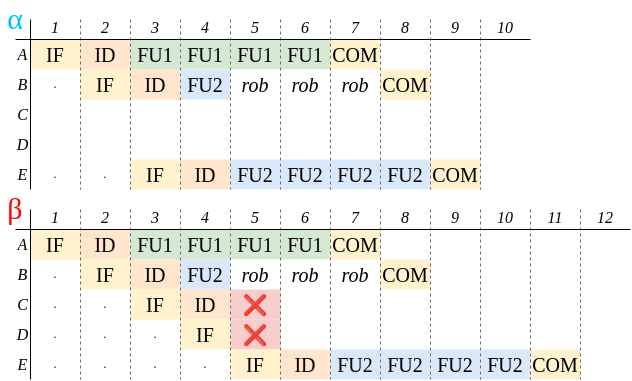
\includegraphics[width=0.8\textwidth]{figures/mispred-intro.png}
	\caption{Pair of traces with correct and incorrect predictions. The squashing event is denoted with a red cross.}
	\label{fig:mispred-intro}
\end{figure}

\TODO{nested mispred region}

\TODO{,ispred region should be sufficiently large}

\subsubsection{Framework Implementation}

We decided to take C++ \cite{stroustrup_c_2015} as an implementation language as it is fast and includes a number of useful data structures in a standard library.


We define a single instruction as follows. It consists of type of FU to be scheduled at (we do not consider resource switch), latency in this FU, set of RAW dependencies. If instruction is a branch, \texttt{mispred\_region} is set to a positive value $n$ denoting the next $n$ instructions are in misprediction region of current instruction. If we want to model only the correct prediction, then \texttt{mispred\_region} is set to 0; this way branch behaves as an ordinary instruction. \texttt{br\_pred} flag specifies if the prediction is correct, which is needed when generating a pair of traces with variation in branch behavior.

\begin{lstlisting}[language=C]
struct Instr {
    int 			fu_type = 0;
    int 			lat_fu = 1;
    std::set<int> 	data_deps;
    int 			mispred_region = 0;
    bool 			br_pred = false;
};
\end{lstlisting}

At the core of our framework is the \texttt{PipelineState} structure, which models the state of all pipeline stages. The \texttt{executed} set tracks instructions that have completed execution in the functional units, enabling dependency resolution. The \texttt{branch\_stack} maintains the context for misprediction regions: each time a branch is fetched, it is pushed onto the stack and remains there until resolved. Together with the \texttt{squashed} set, this mechanism ensures correct handling of mispredicted regions. For simplicity, we do not impose capacity limits on the reservation stations (RS) or reorder buffer (ROB). The \texttt{next()} function advances the pipeline state by one clock cycle and returns whether execution has completed. It operates on the instruction sequence, which is accessed via the program counter (\texttt{pc}).

To obtain an execution trace from a given instruction sequence, we initialize an empty pipeline state (with no instructions present) and repeatedly call \texttt{next()} until the final state is reached. This process yields a sequence of pipeline states, which together form an execution trace.

\begin{lstlisting}[language=C]
struct StageEntry {
    int idx = -1;
    int cycles_left = 0;
};

struct PipelineState {
    int clock_cycle = 0;
    int pc = 0;
    vector<StageEntry> 	stage_IF = 	vector<StageEntry>(SUPERSCALAR);
    vector<int> 		stage_ID = 	vector<int>(SUPERSCALAR);
    vector<set<int>> 	stage_RS = 	vector<set<int>>(FU_NUM);
    vector<StageEntry> 	stage_FU = 	vector<StageEntry>(FU_NUM);
    vector<int> 		stage_COM = vector<int>(SUPERSCALAR);
    deque<int> 			ROB = 		deque<int>();
    set<int> 	executed;
    set<int> 	squashed;
    vector<int> branch_stack;

    bool next(const vector<Instr>& prog);
};
\end{lstlisting}

To enable efficient exploration of trace pairs that demonstrate timing anomalies (TA) and to support analysis over larger state spaces, not limited to a fixed instruction trace template, the framework provides three operating modes:

\begin{enumerate}
	\item \textbf{Manual mode}: The user provides an instruction trace in the format given above. The framework then generates the corresponding pair of execution traces. This mode enables rapid construction and analysis of custom scenarios.
	\item \textbf{Random search}: The framework generates random instruction traces within user-defined constraints and checks the resulting execution traces against a specified property. For example, it can explore all traces of length 5 containing one branch instruction and at most two RAW dependencies. While this method cannot guarantee exhaustive coverage of the state space, it is effective for quickly finding counterexamples in large spaces.
	\item \textbf{State exploration}: The trace template is specified as a generator function, similar to random search mode. The framework then exhaustively verifies the property on every possible input, ensuring complete state space coverage. This mode is useful for proving properties about the model, but may be inefficient for finding counterexamples in large spaces due to the potential for excessive exploration of uninteresting subspaces.
\end{enumerate}


In summary, we created a tool capable of studying traces both in automated and guided way. Our time-efficient implementation enables exploration of significantly larger state spaces that are infeasible to analyze using Binder's original framework. While TLA$^+$ offers greater expressive power for formalizing properties such as leveraging temporal logic, in the context of Binder et al., the verified property was ultimately specified as a state predicate embedded in Python code. Therefore, we believe that our choice of implementation does not result in a substantial loss of expressiveness or rigor for the intended analyses.

\section{Generating TA Examples}

TODO: describe the setting, the search space given to the tool to produce an example (comment on performance "example was found in ... ms", "... examples were found"). Explain why examples show TA

We start with generating representative examples of branch-caused TA. The hypothesis is that the correct branch prediction may yield a longer execution than the same setting with misprediction. We want to have a simple example, thus decided we perform an exhaustive search in a state of the programs with:

\begin{enumerate}
    \item 4 committed instructions with;
    \item At most 2 dependencies;
    \item 1 branch instruction.
\end{enumerate}

The latency of branch instruction was chosen to be $1$ as conditionals jumps often require simple one-cycle operations (such as equality, more or equal, less or equal, etc.). The latencies of other instructions in the chosen setting are $4$. We have chosen single-scalar pipeline with 2 FUs.

Our framework explored $4608$ input traces in around $150$ ms: among those 2 TAs were identified, explained in Examples \ref{ex:bp-ta} and \ref{ex:bp-ta-1}.

\begin{example}
Figure \ref{fig:bp-ta-inputs-0} shows an instruction trace found from generating random examples. $C$ is a branch with misprediction region ${D, E}$. There is one dependency: $A \rightarrow B$. Figure \ref{fig:bp-ta-traces-0} shows the associated pair of execution traces. In trace $\alpha$ instructions $D$ and $E$ as skipped due to the correct prediction, so $F$ is fetched right away. This causes an earlier execution of $F$, which leads to $FU2$ being busy at clock cycle $7$ and therefore instruction $B$ starts being executed later, thus causing a slowdown.

\label{ex:bp-ta}
\end{example}

\begin{example}
The other TA which input and execution trace are shown in Figures \ref{fig:bp-ta-inputs-1} and \ref{fig:bp-ta-traces-1} respectively is different from Example \ref{ex:bp-ta} only by the FU of instruction $C$ while the other instructions are the same (also the misprediction region is longer due to longer delay between branch prediction and branch resolution).
\label{ex:bp-ta-1}
\end{example}


\begin{figure}[H]
    \centering
    \begin{subfigure}[b]{0.45\textwidth}
        \centering
        \begin{tabular}{rr|ccc}
            &  & Res. & Dep. & Lat. \\ \hline
            \textit{A:} &  & FU1 &  & $4$ \\
            \textit{B:} &  & FU2 & $\{A\}$ & $4$ \\
            \textit{*C:} &  & \textbf{FU2} &  & $1$ \\
            & \textit{D:} & FU1 &  & $4$ \\
            & \textit{E:} & FU1 &  & $4$ \\
            \textit{H:} &  & FU2 &  & $4$ \\
        \end{tabular}
        \caption{Input from Example \ref{ex:bp-ta}}
        \label{fig:bp-ta-inputs-0}
    \end{subfigure}
    \hfill
    \begin{subfigure}[b]{0.45\textwidth}
        \centering
        
        \begin{tabular}{rr|ccc}
            &  & Res. & Dep. & Lat. \\ \hline
            \textit{A:} &  & FU1 &  & $4$ \\
            \textit{B:} &  & FU2 & $\{A\}$ & $4$ \\
            \textit{*C:} &  & \textbf{FU1} &  & $1$ \\
            & \textit{D:} & FU1 &  & $4$ \\
            & \textit{E:} & FU1 &  & $4$ \\
            & \textit{F:} & FU1 &  & $4$ \\
            & \textit{G:} & FU1 &  & $4$ \\
            \textit{H:} &  & FU2 &  & $4$ \\
        \end{tabular}
        \caption{Input from Example \ref{ex:bp-ta-1}}
        \label{fig:bp-ta-inputs-1}
    \end{subfigure}
    \caption{Two anomalous inputs found from the setting}
    \label{fig:bp-ta-inputs}
\end{figure}



\begin{figure}[H]
    \centering
    \begin{subfigure}[b]{0.49\textwidth}
        \centering
        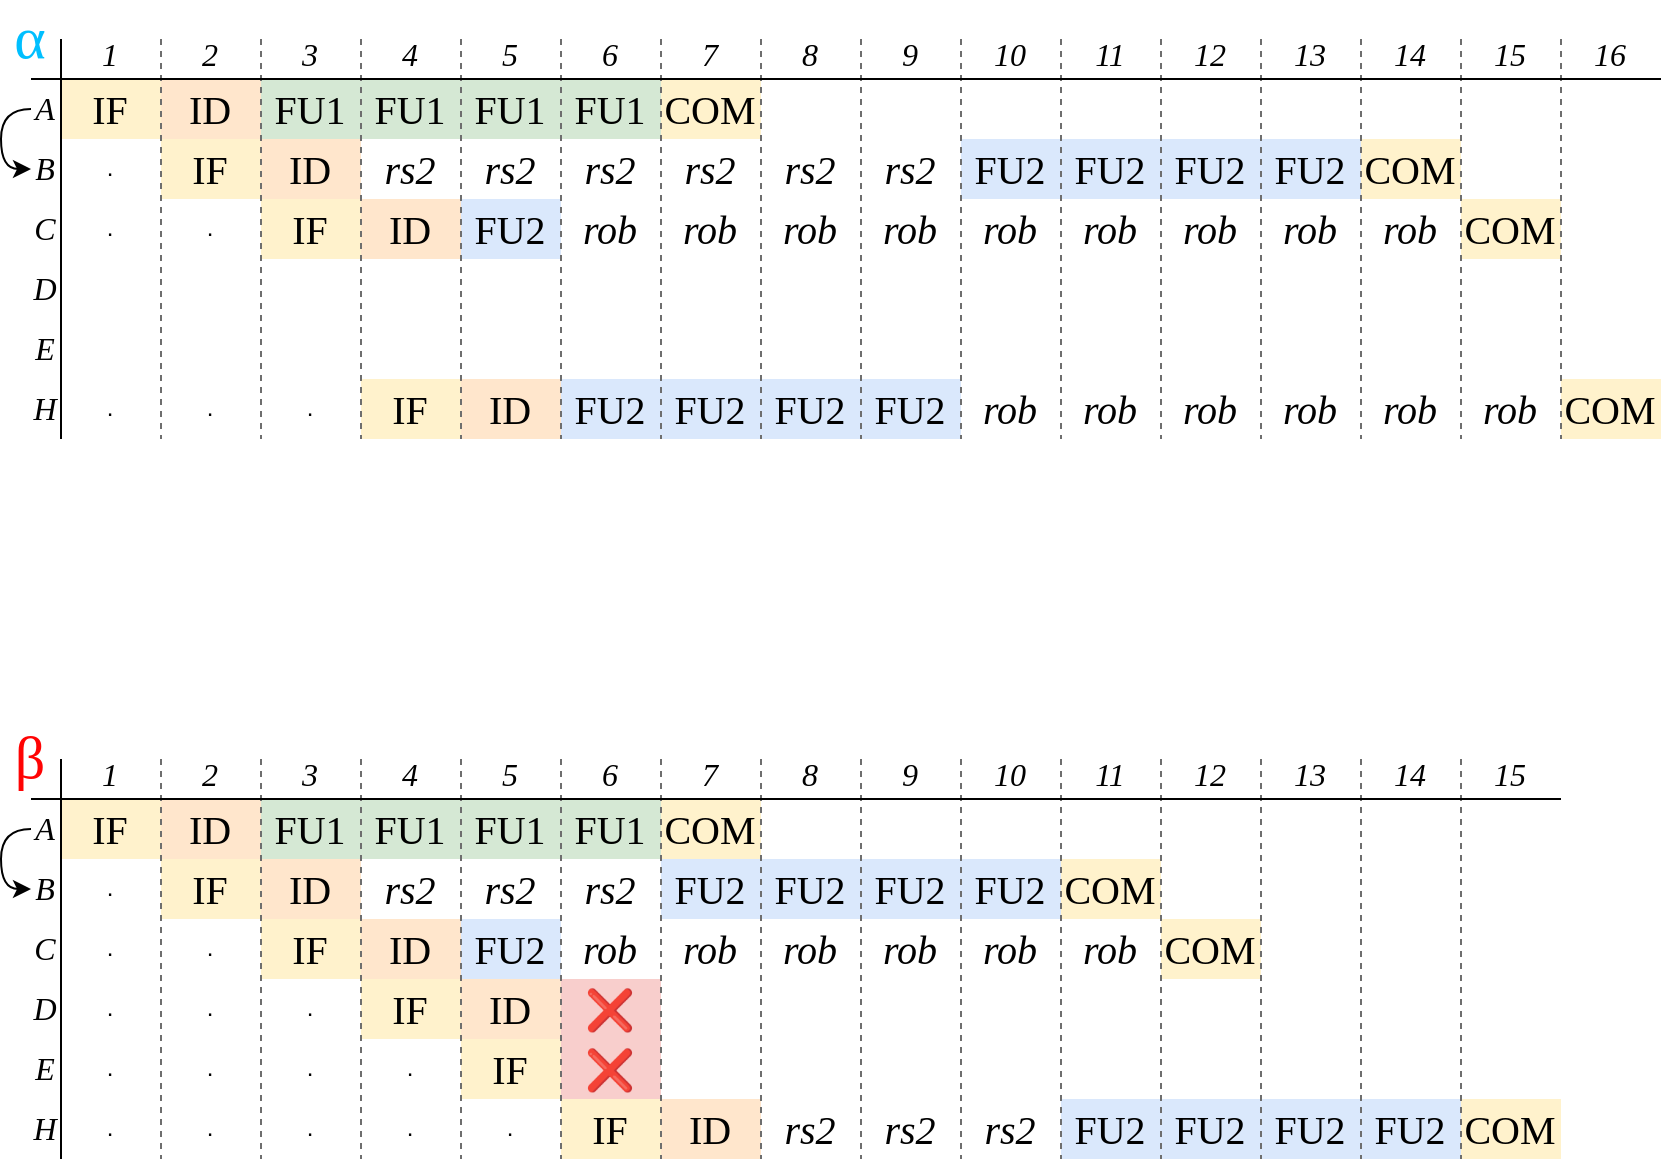
\includegraphics[width=\textwidth]{figures/simple-branch-ta.png}
        \caption{Trace from Example \ref{ex:bp-ta}}
        \label{fig:bp-ta-traces-0}
    \end{subfigure}
    \hfill
    \begin{subfigure}[b]{0.49\textwidth}
        \centering
        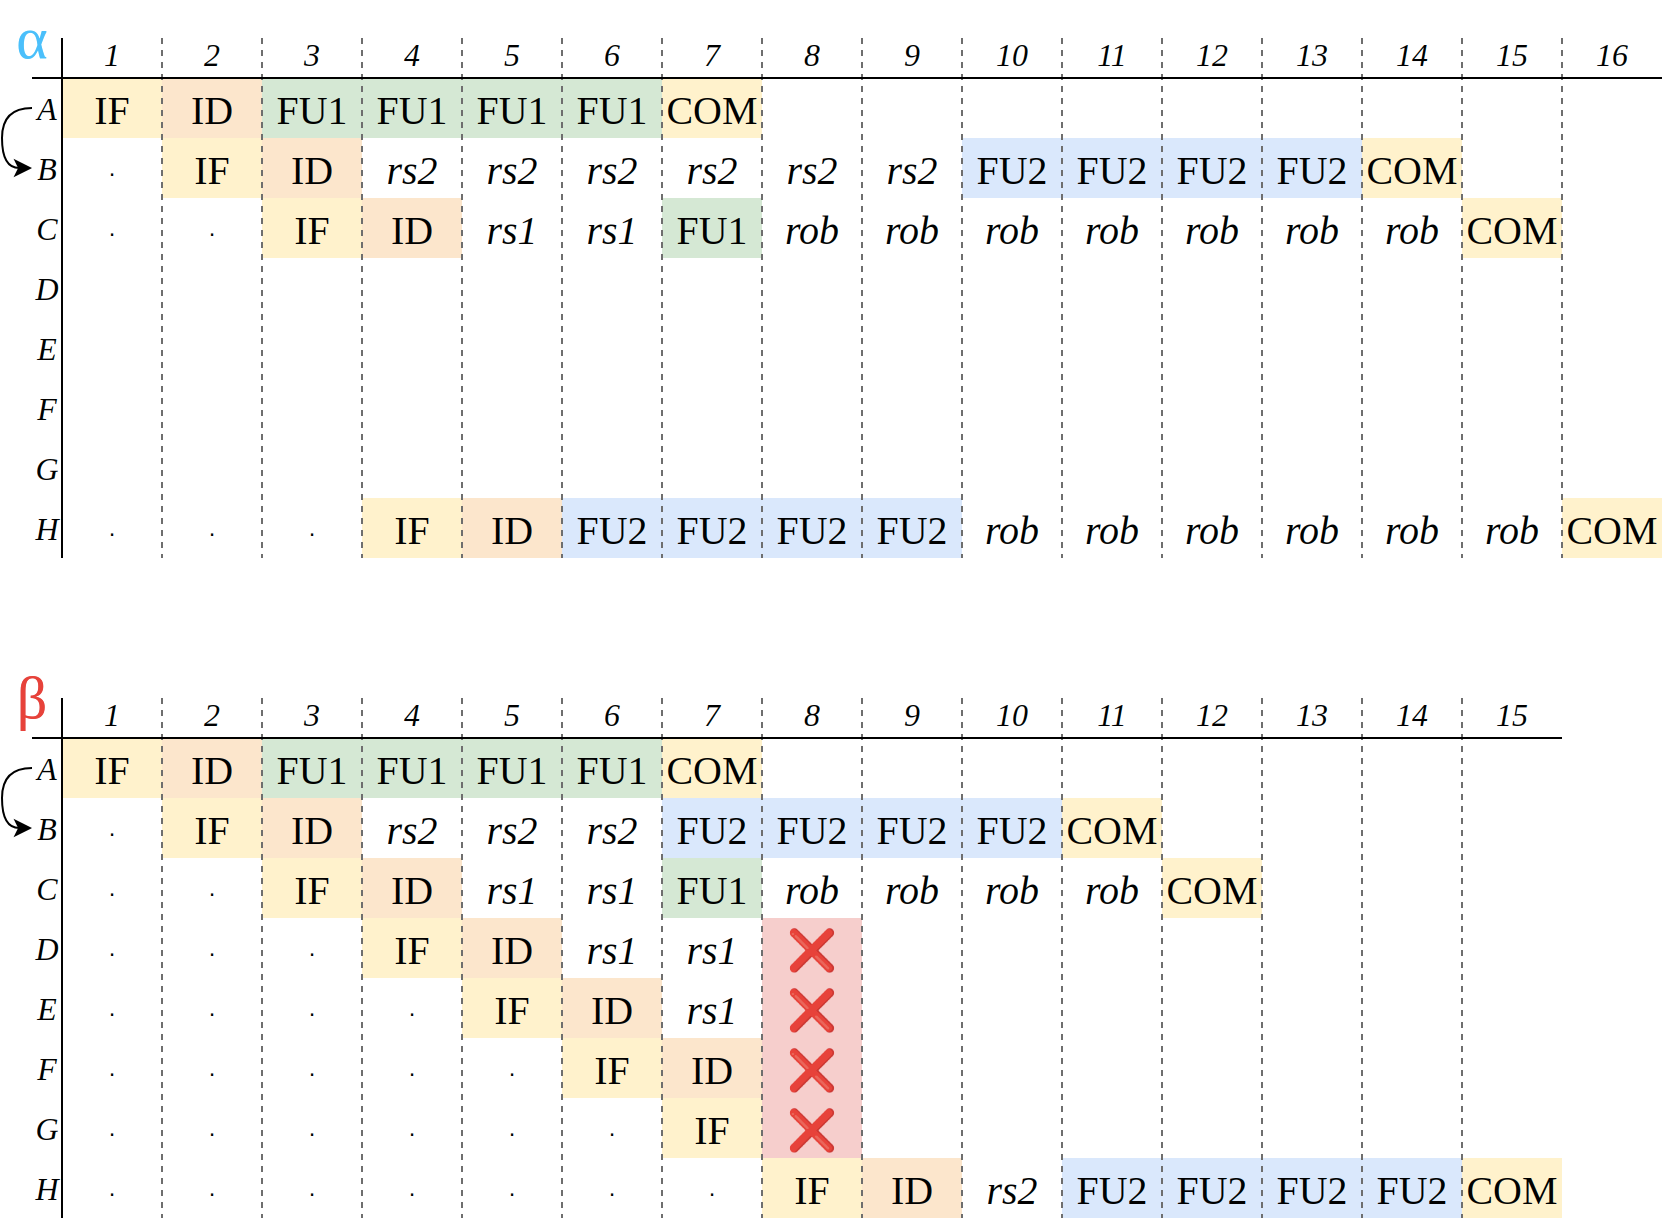
\includegraphics[width=\textwidth]{figures/simple-branch-ta-1.png}
        \caption{Trace from Example \ref{ex:bp-ta-1}}
        \label{fig:bp-ta-traces-1}
    \end{subfigure}
    \caption{Two TA traces found by the framework}
    \label{fig:bp-ta-traces}
\end{figure}

The only essential difference between Examples \ref{ex:bp-ta} and \ref{ex:bp-ta-1} is the length of misprediction region. The scheduling of instructions $A$, $B$ and $H$ is exactly the same in the two examples. This gives us a hint that some anomalies may fall down in the same category which can give us a classification of TAs.

Another notable observation is that here the anomalous effect can be explained by just by the later fetch of instruction $H$. Interestingly, the same effect can be obtained by modeling a cache miss for the fetch of $H$ as shown in Figure \ref{fig:equiv-to-bp-ta}. Here, int both $\alpha$ and $\beta$ the prediction is correct, however, there is a cache hit in $\alpha$ and cache miss in $\beta$.

TODO: TA only on commit; no longer effect?

\begin{figure}[H]
    \centering
    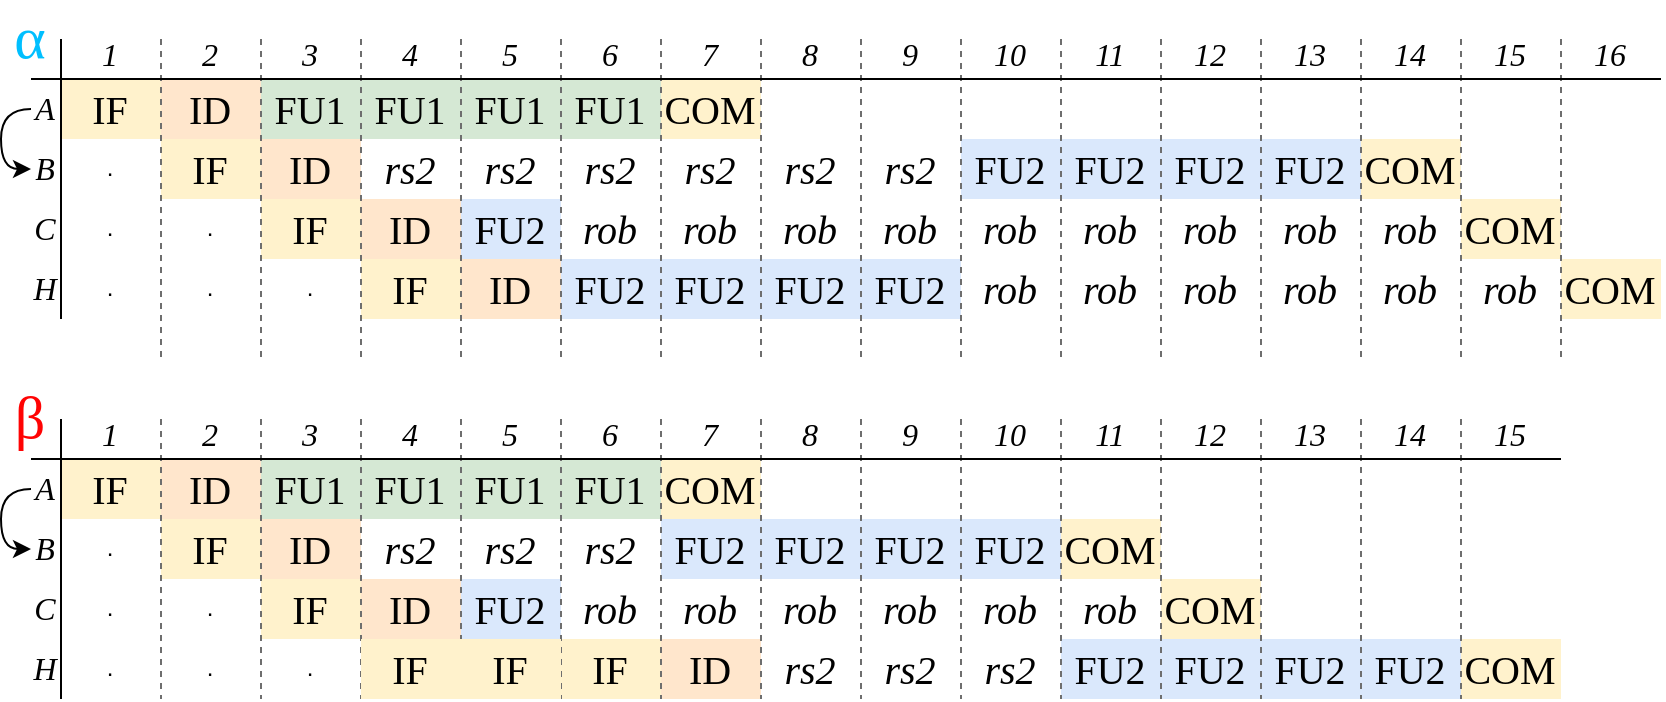
\includegraphics[width=\textwidth]{figures/equiv-trace.png}
    \caption{Cache miss on fetch of $H$ causing the same effect as branch misprediction}
    \label{fig:equiv-to-bp-ta}
\end{figure}

\section{Formalizing Definition}

TODO: start with latency, show it on example, formalize an assumption: show new contradicting examples

For ex 2 3 BInder's def works ...

but what dfo we do if smth inside of spec region?

\TODO{introdcue letters for instructions to make things clear}

Since there exist an equivalent behavior (shown at Figure \ref{fig:equiv-to-bp-ta}) to Examples \ref{ex:bp-ta}  and \ref{ex:bp-ta-1}, it should be possible to adapt Binder's definition for these cases. Let us take an Example \ref{ex:bp-ta}. In Binder's definition the source of TA is a variation, thus it must be defined first. In trace showing equivalent behavior (Figure \ref{fig:equiv-to-bp-ta}) the variation is in IF latency i.e. the delay between $\IFa$ and $\IFr$. In the Example \ref{ex:bp-ta} both $\IFa$ and $\IFr$ are different between traces $\alpha$ and $\beta$ thus the same variation can not be used. We may use the fact that for a given instruction $\IFa$ coincides with $\IFr$ of previous instruction and use this $\IFr$ as the start of the latency. Thus, the latency can be measured between $\IFr$ of branch instruction and $\IFr$ of first instruction after misprediction region.

However, we still need to take into account other variations, so the possible variation in IF of the after-branch instruction will be mixed with branch-related variation as their latencies overlap. So instead we propose using two events to signify the variation:

\begin{enumerate}
    \item \textbf{Branch Prediction (BP)} -- moment when prediction happens and speculative executions starts;
    \item \textbf{Correct Branch Taken (BT)} -- the instruction from correct branch enters the pipeline.
\end{enumerate}

Note that $BP$ corresponds to $\IFr$ of branch instruction and $BT$ is $\IFa$ of a first instruction after misprediction region of the branch. In case of a single variation that is in branch prediction, the TA pattern is detected in the same way as shown in Figure \ref{fig:equiv-to-bp-ta}, but with latency being shorter by 1 clock cylce (\TODO{or more...}) and the delay being longer by the same value.

Figure \ref{fig:bp-ta-analysed} shows this idea applied to Example \ref{ex:bp-ta}. Both latencies corresponding to variation are 1 clock cycle shorter compared to example shown in Figure \ref{fig:equiv-to-bp-ta}. The causality region also starts 1 clock cycle earlier, however is still going through the same events. Note here that we do not need any additional rules to build causality arcs.

A major assumption that allowed us to adapt the definition is that the branch behavior is just postponing the fetch of instruction following misprediction region. In this case the behavior can be compared to the effect of cache miss in IF stage -- this is also not completely true, as the penalty for cache miss is fixed while the size of misprediction region depends on the time between the prediction and the resolution of the branch. Therefore, in the rest of the article we focus more on examples that do not fit the assumption.

\TODO{Bound the effect of branch resolution?}

\begin{figure}[H]
    \centering
    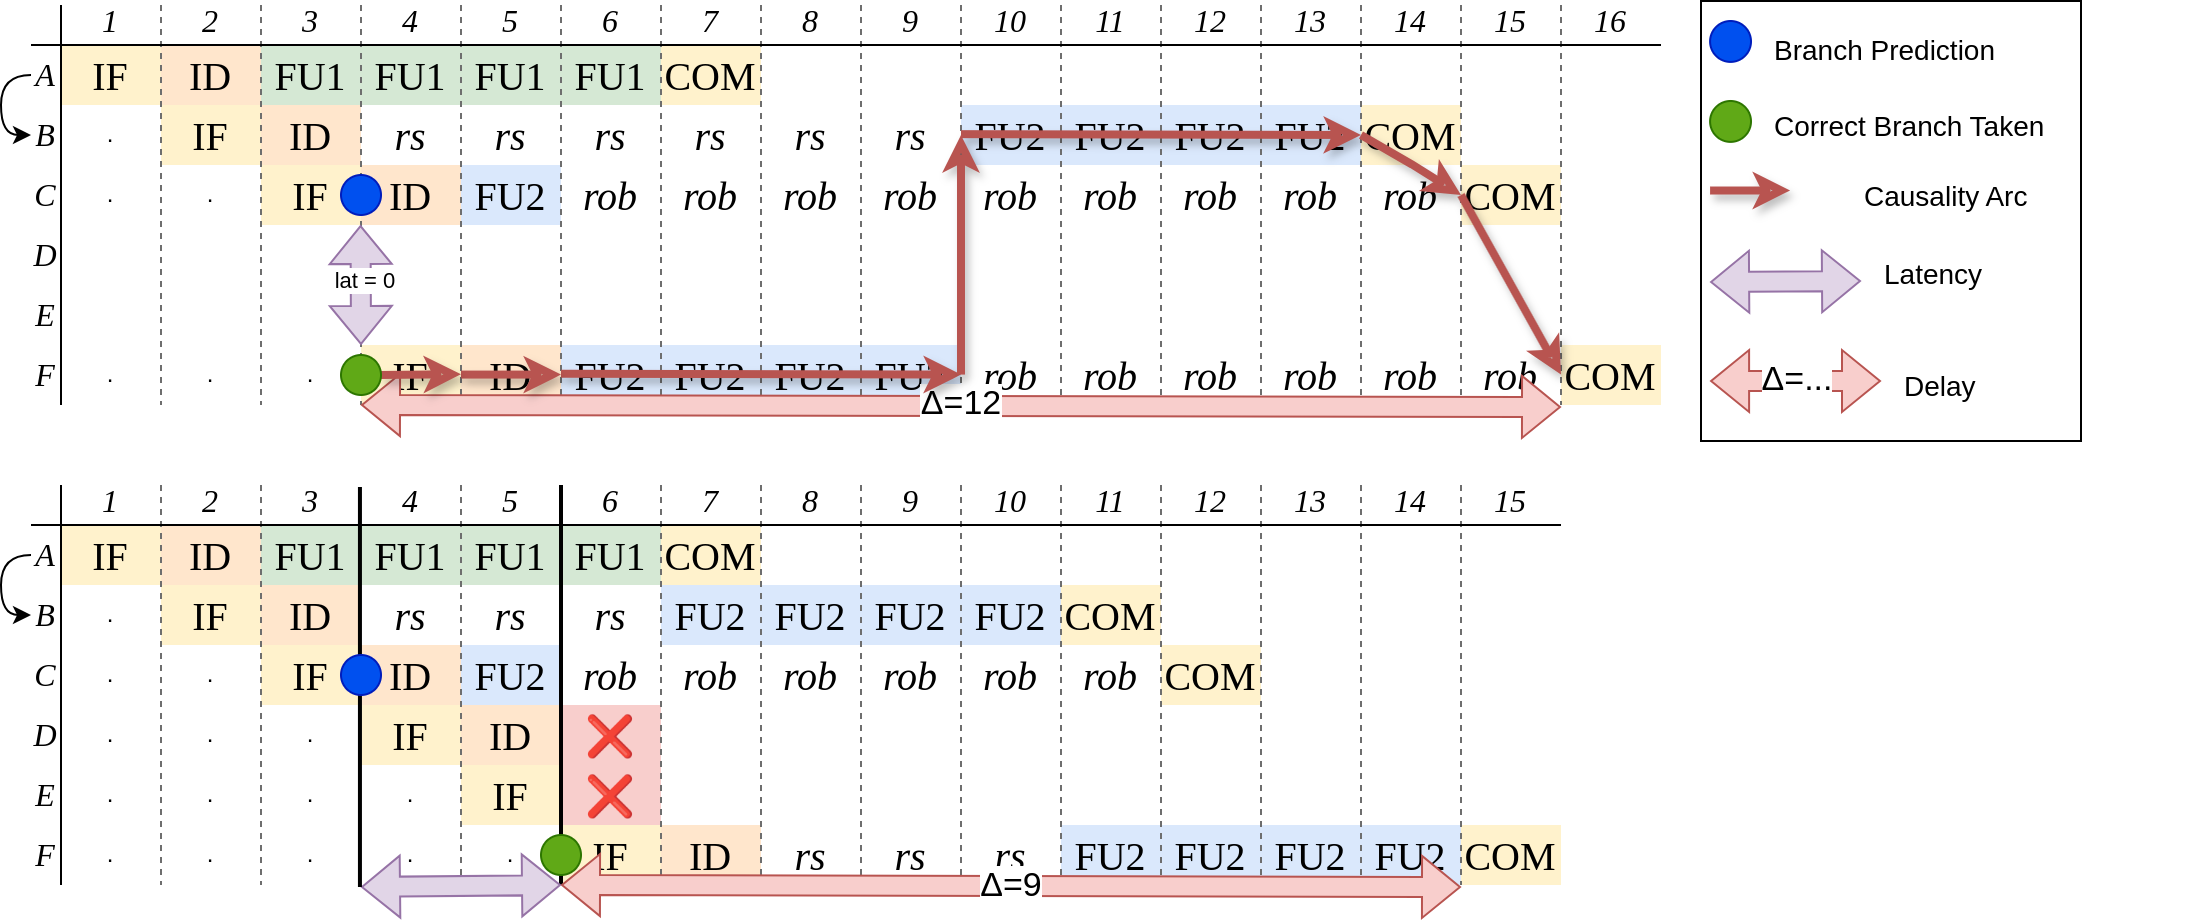
\includegraphics[width=\textwidth]{figures/simple-branch-ta-analysed.png}
    \caption{\TODO{}}
    \label{fig:bp-ta-analysed}
\end{figure}

\subsection{More complex examples}



\section{Gap problem}

\subsection{Problem statement}

TODO: explain that even without branching there is a problem

\subsection{Requirements for Causality Graph}

TODO: formalize properties that we expect from causality graph and explain why they are violated

\subsection{Towards New Causality Definition}

TODO: propose a method that can be used to construct a "true causality" graph: set of constraints, moving events around